\documentclass[12pt]{article}

\usepackage{amsmath}
\usepackage{array}
\usepackage{caption}
\usepackage[top=1in, bottom=1in, left=0.75in, right=0.75in]{geometry}
\usepackage{graphicx}
\usepackage[colorlinks=true, allcolors=blue]{hyperref}
\usepackage[utf8]{inputenc}
\usepackage{multirow}
\usepackage{pdfpages}
\usepackage[section]{placeins}

\graphicspath{{figures/}}

\title{ECE 271: Chapter 5 Reading Report}
\author{Phi Luu}
\date{November 12\textsuperscript{th}, 2018}

\begin{document}

\maketitle

%%%%%%%%%%%%%%%%%%%%%%%%%%%%%%%%%%%%%%%%%%%%%%%%%%%%%%%%%%%%%%%%%%%%%%%%%%%%%%%%
% Chapter Outline
%%%%%%%%%%%%%%%%%%%%%%%%%%%%%%%%%%%%%%%%%%%%%%%%%%%%%%%%%%%%%%%%%%%%%%%%%%%%%%%%
\section{Chapter Outline}

%%%%%%%%%%%%%%%%%%%%%%%%%%%%%%%%%%%%%%%%
% Introduction
%%%%%%%%%%%%%%%%%%%%%%%%%%%%%%%%%%%%%%%%
\subsection{Introduction}

%%%%%%%%%%%%%%%%%%%%%%%%%%%%%%%%%%%%%%%%
% Arithmetic Circuits
%%%%%%%%%%%%%%%%%%%%%%%%%%%%%%%%%%%%%%%%
\subsection{Arithmetic Circuits}

\begin{enumerate}
  %%%%%%%%%%%%%%%%%%%%
  % Addition
  %%%%%%%%%%%%%%%%%%%%
  \item \textbf{Addition}

  %%%%%%%%%%%%%%%%%%%%
  % Subtraction
  %%%%%%%%%%%%%%%%%%%%
  \item \textbf{Subtraction}

  %%%%%%%%%%%%%%%%%%%%
  % Comparators
  %%%%%%%%%%%%%%%%%%%%
  \item \textbf{Comparators}

  %%%%%%%%%%%%%%%%%%%%
  % ALU
  %%%%%%%%%%%%%%%%%%%%
  \item \textbf{ALU}

  %%%%%%%%%%%%%%%%%%%%
  % Shifters and Rotators
  %%%%%%%%%%%%%%%%%%%%
  \item \textbf{Shifters and Rotators}

  %%%%%%%%%%%%%%%%%%%%
  % Multiplication
  %%%%%%%%%%%%%%%%%%%%
  \item \textbf{Multiplication}

  %%%%%%%%%%%%%%%%%%%%
  % Division
  %%%%%%%%%%%%%%%%%%%%
  \item \textbf{Division}

  %%%%%%%%%%%%%%%%%%%%
  % Further Reading
  %%%%%%%%%%%%%%%%%%%%
  \item \textbf{Further Reading}
\end{enumerate}

%%%%%%%%%%%%%%%%%%%%%%%%%%%%%%%%%%%%%%%%
% Number Systems
%%%%%%%%%%%%%%%%%%%%%%%%%%%%%%%%%%%%%%%%
\subsection{Number Systems}

\begin{enumerate}
  %%%%%%%%%%%%%%%%%%%%
  % Fixed-Point Number Systems
  %%%%%%%%%%%%%%%%%%%%
  \item \textbf{Fixed-Point Number Systems}

  %%%%%%%%%%%%%%%%%%%%
  % Floating-Point Number Systems
  %%%%%%%%%%%%%%%%%%%%
  \item \textbf{Floating-Point Number Systems}
\end{enumerate}

%%%%%%%%%%%%%%%%%%%%%%%%%%%%%%%%%%%%%%%%
% Sequential Building Blocks
%%%%%%%%%%%%%%%%%%%%%%%%%%%%%%%%%%%%%%%%
\subsection{Sequential Building Blocks}

\begin{enumerate}
  %%%%%%%%%%%%%%%%%%%%
  % Counters
  %%%%%%%%%%%%%%%%%%%%
  \item \textbf{Counters}

  %%%%%%%%%%%%%%%%%%%%
  % Shift Registers
  %%%%%%%%%%%%%%%%%%%%
  \item \textbf{Shift Registers}
\end{enumerate}

%%%%%%%%%%%%%%%%%%%%%%%%%%%%%%%%%%%%%%%%
% Memory Arrays
%%%%%%%%%%%%%%%%%%%%%%%%%%%%%%%%%%%%%%%%
\subsection{Memory Arrays}

\begin{enumerate}
  %%%%%%%%%%%%%%%%%%%%
  % Overview
  %%%%%%%%%%%%%%%%%%%%
  \item \textbf{Overview}

  %%%%%%%%%%%%%%%%%%%%
  % Dynamic Random Access Memory (DRAM)
  %%%%%%%%%%%%%%%%%%%%
  \item \textbf{Dynamic Random Access Memory (DRAM)}

  %%%%%%%%%%%%%%%%%%%%
  % Static Random Access Memory (SRAM)
  %%%%%%%%%%%%%%%%%%%%
  \item \textbf{Static Random Access Memory (SRAM)}

  %%%%%%%%%%%%%%%%%%%%
  % Area and Delay
  %%%%%%%%%%%%%%%%%%%%
  \item \textbf{Area and Delay}

  %%%%%%%%%%%%%%%%%%%%
  % Register Files
  %%%%%%%%%%%%%%%%%%%%
  \item \textbf{Register Files}

  %%%%%%%%%%%%%%%%%%%%
  % Read Only Memory
  %%%%%%%%%%%%%%%%%%%%
  \item \textbf{Read Only Memory}

  %%%%%%%%%%%%%%%%%%%%
  % Logic Using Memory Arrays
  %%%%%%%%%%%%%%%%%%%%
  \item \textbf{Logic Using Memory Arrays}

  %%%%%%%%%%%%%%%%%%%%
  % Memory HDL
  %%%%%%%%%%%%%%%%%%%%
  \item \textbf{Memory HDL}
\end{enumerate}

%%%%%%%%%%%%%%%%%%%%%%%%%%%%%%%%%%%%%%%%
% Logic Arrays
%%%%%%%%%%%%%%%%%%%%%%%%%%%%%%%%%%%%%%%%
\subsection{Logic Arrays}

\begin{enumerate}
  %%%%%%%%%%%%%%%%%%%%
  % Programmable Logic Array
  %%%%%%%%%%%%%%%%%%%%
  \item \textbf{Programmable Logic Array}

  %%%%%%%%%%%%%%%%%%%%
  % Field Programmable Gate Array
  %%%%%%%%%%%%%%%%%%%%
  \item \textbf{Field Programmable Gate Array}

  %%%%%%%%%%%%%%%%%%%%
  % Array Implementation
  %%%%%%%%%%%%%%%%%%%%
  \item \textbf{Array Implementation}
\end{enumerate}

%%%%%%%%%%%%%%%%%%%%%%%%%%%%%%%%%%%%%%%%
% Summary
%%%%%%%%%%%%%%%%%%%%%%%%%%%%%%%%%%%%%%%%
\subsection{Summary}

%%%%%%%%%%%%%%%%%%%%%%%%%%%%%%%%%%%%%%%%%%%%%%%%%%%%%%%%%%%%%%%%%%%%%%%%%%%%%%%%
% Grey Box Exploration
%%%%%%%%%%%%%%%%%%%%%%%%%%%%%%%%%%%%%%%%%%%%%%%%%%%%%%%%%%%%%%%%%%%%%%%%%%%%%%%%
\section{Grey Box Exploration}

\begin{enumerate}
  %%%%%%%%%%%%%%%%%%%%%%%%%%%%%%%%%%%%%%%%
  % First grey box
  %%%%%%%%%%%%%%%%%%%%%%%%%%%%%%%%%%%%%%%%
  \item The first blurb is on page , which states \textit{}

  %%%%%%%%%%%%%%%%%%%%%%%%%%%%%%%%%%%%%%%%
  % Second grey box
  %%%%%%%%%%%%%%%%%%%%%%%%%%%%%%%%%%%%%%%%
  \item The second blurb is on page , which states \textit{}
\end{enumerate}

%%%%%%%%%%%%%%%%%%%%%%%%%%%%%%%%%%%%%%%%%%%%%%%%%%%%%%%%%%%%%%%%%%%%%%%%%%%%%%%%
% Figures
%%%%%%%%%%%%%%%%%%%%%%%%%%%%%%%%%%%%%%%%%%%%%%%%%%%%%%%%%%%%%%%%%%%%%%%%%%%%%%%%
\section{Figures}

Two figures were selected from this chapter for special recognition. Figure was selected because

% \begin{figure}[ht]
%     \centering
%     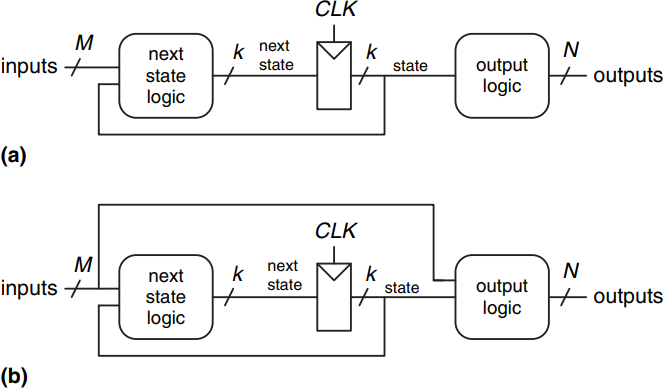
\includegraphics[width=0.5\textwidth]{moore_and_mealy_fsm.png}
%     \caption{Finite state machines: (a) Moore machine, (b) Mealy machine}
%     \label{figure:13}
% \end{figure}

Figure was selected because

% \begin{figure}[ht]
%     \centering
%     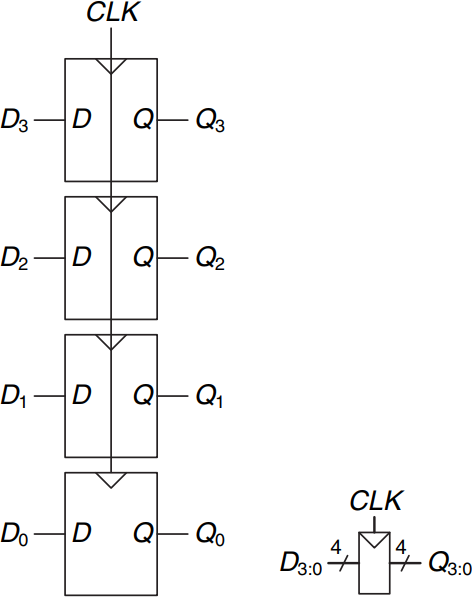
\includegraphics[width=0.25\textwidth]{register_4bit.png}
%     \caption{Inside of a 4-bit register}
%     \label{figure:14}
% \end{figure}

%%%%%%%%%%%%%%%%%%%%%%%%%%%%%%%%%%%%%%%%%%%%%%%%%%%%%%%%%%%%%%%%%%%%%%%%%%%%%%%%
% Example Problems
%%%%%%%%%%%%%%%%%%%%%%%%%%%%%%%%%%%%%%%%%%%%%%%%%%%%%%%%%%%%%%%%%%%%%%%%%%%%%%%%
\section{Example Problems}

See the attached images on the next four pages.

% 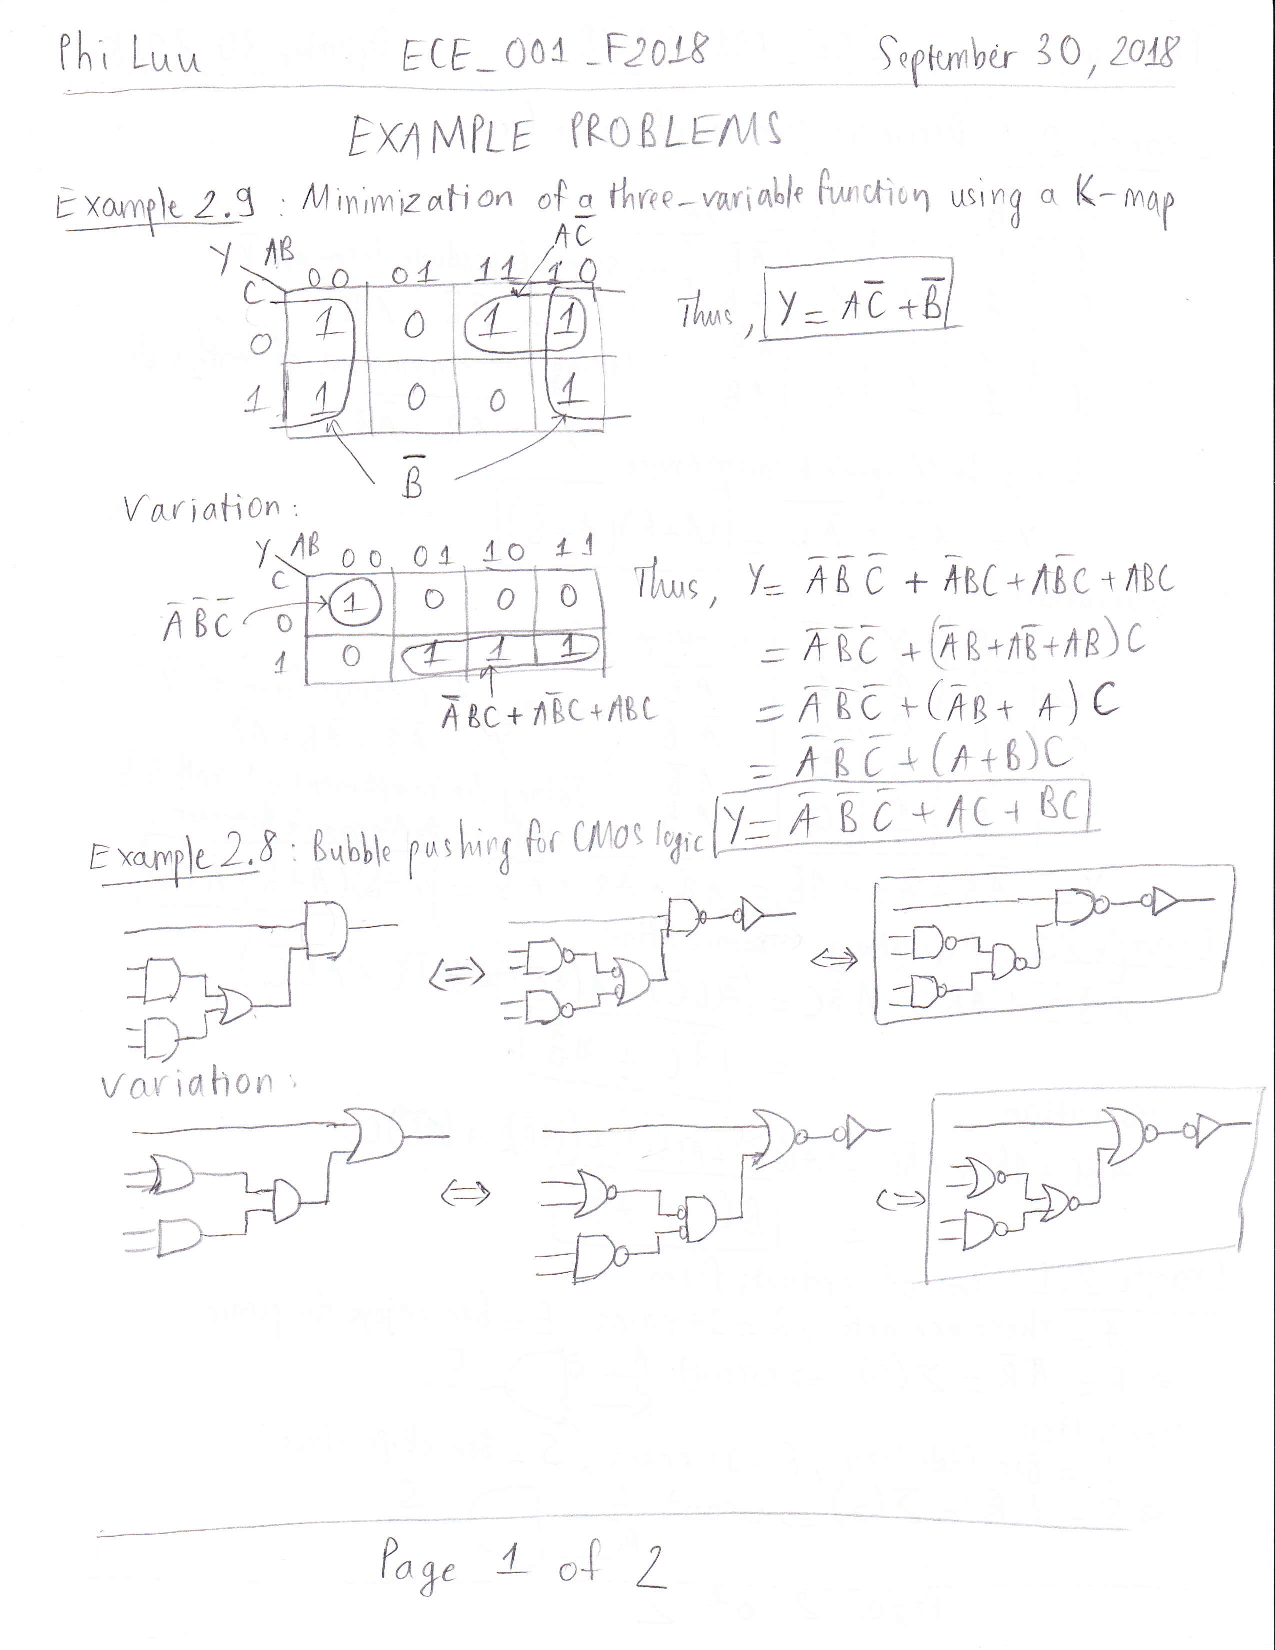
\includepdf[page=-]{example_problems}

%%%%%%%%%%%%%%%%%%%%%%%%%%%%%%%%%%%%%%%%%%%%%%%%%%%%%%%%%%%%%%%%%%%%%%%%%%%%%%%%
% Glossary
%%%%%%%%%%%%%%%%%%%%%%%%%%%%%%%%%%%%%%%%%%%%%%%%%%%%%%%%%%%%%%%%%%%%%%%%%%%%%%%%
\section{Glossary}

All definitions were found from the Google search engine, typing "define arithmetic logic unit" for the first item.

\begin{enumerate}
  \item Arithmetic Logic Unit (ALU)

  noun:

  \begin{enumerate}
    \item A unit in a computer that carries out arithmetic and logical operations.
  \end{enumerate}

  \item Comparator

  noun:

  \begin{enumerate}
    \item a device for comparing a measurable property or thing with a reference or standard.

    \begin{itemize}
      \item an electronic circuit for comparing two electrical signals.
      \item something used as a standard for comparison.
    \end{itemize}
  \end{enumerate}

  \item{Read Only Memory}

  noun:

  \begin{enumerate}
    \item {[computing]} memory read at high speed but not capable of being changed by program instructions.
  \end{enumerate}

  \item{Array}

  noun:

  \begin{enumerate}
    \item an impressive display or range of a particular type of thing.

    \item an ordered series or arrangement.
      \begin{itemize}
        \item an arrangement of troops.
        \item {[mathematics]} an arrangement of quantities or symbols in rows and columns; a matrix.
        \item {[computing]} an indexed set of related elements.
      \end{itemize}

    \item {[literary]} elaborate or beautiful clothing.
    \item {[law]} a list of jurors empaneled.
  \end{enumerate}

  verb:

  \begin{enumerate}
    \item display or arrange (things) in a particular way.
    \item dress someone in (the clothes specified).
    \item {[law]} empanel (a jury).
  \end{enumerate}

  \item{Random Access}

  noun:

  \begin{enumerate}
    \item {[computing]} the process of transferring information to or from memory in which every memory location can be accessed directly rather than being accessed in a fixed sequence.
  \end{enumerate}
\end{enumerate}

%%%%%%%%%%%%%%%%%%%%%%%%%%%%%%%%%%%%%%%%%%%%%%%%%%%%%%%%%%%%%%%%%%%%%%%%%%%%%%%%
% Interview Question
%%%%%%%%%%%%%%%%%%%%%%%%%%%%%%%%%%%%%%%%%%%%%%%%%%%%%%%%%%%%%%%%%%%%%%%%%%%%%%%%
\section{Interview Question}

See the attached image on the next page.

% 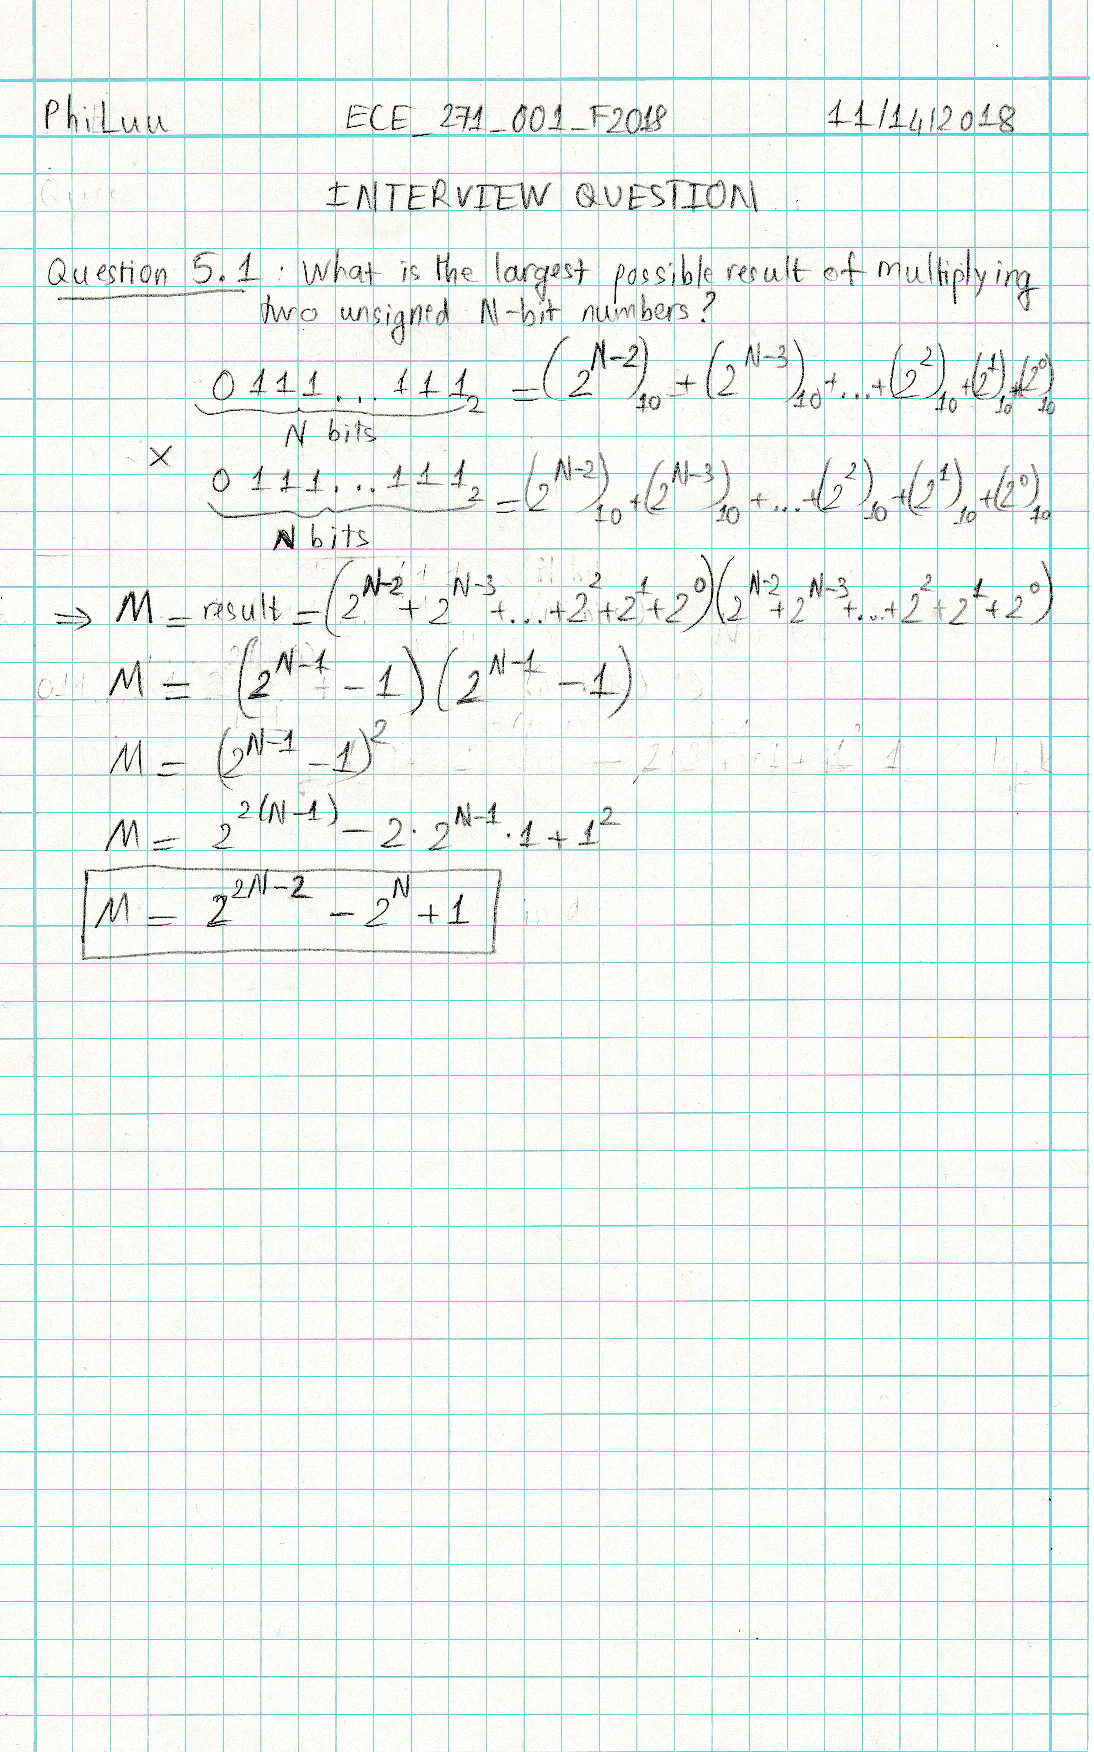
\includepdf[page=-]{interview_question}

%%%%%%%%%%%%%%%%%%%%%%%%%%%%%%%%%%%%%%%%%%%%%%%%%%%%%%%%%%%%%%%%%%%%%%%%%%%%%%%%
% Reflection
%%%%%%%%%%%%%%%%%%%%%%%%%%%%%%%%%%%%%%%%%%%%%%%%%%%%%%%%%%%%%%%%%%%%%%%%%%%%%%%%
\section{Reflection}

%%%%%%%%%%%%%%%%%%%%%%%%%%%%%%%%%%%%%%%%%%%%%%%%%%%%%%%%%%%%%%%%%%%%%%%%%%%%%%%%
% Questions for Lecture
%%%%%%%%%%%%%%%%%%%%%%%%%%%%%%%%%%%%%%%%%%%%%%%%%%%%%%%%%%%%%%%%%%%%%%%%%%%%%%%%
\section{Questions for Lecture}

\begin{enumerate}
  \item
  \item
  \item
\end{enumerate}

\end{document}
